\documentclass[a4paper,12pt]{article}
%%%%%%%%%%%%%%%%%%%%%%%%%%%%%%%%%%%%%%%%%%%%%%%%%%%%%%%%%%%%%%%%%%%%%%%%%%%%%%%%%%%%%%%%%%%%%%%%%%%%%%%%%%%%%%%%%%%%%%%%%%%%%%%%%%%%%%%%%%%%%%%%%%%%%%%%%%%%%%%%%%%%%%%%%%%%%%%%%%%%%%%%%%%%%%%%%%%%%%%%%%%%%%%%%%%%%%%%%%%%%%%%%%%%%%%%%%%%%%%%%%%%%%%%%%%%
\usepackage{eurosym}
\usepackage{vmargin}
\usepackage{amsmath}
\usepackage{graphics}
\usepackage{epsfig}
\usepackage{subfigure}
\usepackage{fancyhdr}
%\usepackage{listings}
\usepackage{framed}
\usepackage{graphicx}

\setcounter{MaxMatrixCols}{10}
%TCIDATA{OutputFilter=LATEX.DLL}
%TCIDATA{Version=5.00.0.2570}
%TCIDATA{<META NAME="SaveForMode" CONTENT="1">}
%TCIDATA{LastRevised=Wednesday, February 23, 2011 13:24:34}
%TCIDATA{<META NAME="GraphicsSave" CONTENT="32">}
%TCIDATA{Language=American English}

\pagestyle{fancy}
\setmarginsrb{20mm}{0mm}{20mm}{25mm}{12mm}{11mm}{0mm}{11mm}
\lhead{Control Charts} \rhead{Kevin O'Brien}
\chead{Statistical Quality Control}
%\input{tcilatex}
\begin{document}
\tableofcontents
\newpage

%------------------------------------------------------------- %

\section{Control Chart}
\begin{itemize}
\item A control chart is a graphical representation of a characteristic of a process, showing plotted values of some statistic, a central line, and one or two control limits. \item It is used to determine whether a process has been operating in statistical control and is an aid to maintaining statistical control.
\end{itemize}


\newpage
\section{Control Chart Selection}
\begin{itemize}
\item Correct control chart selection is a critical part of creating a control chart. If the wrong control chart is selected, the control limits will not be correct for the data. 
\item The type of control chart required is determined by the type of data to be plotted and the format in which it is collected. \item Data collected is either in variables or attributes format, and the amount of data contained in each sample (subgroup) collected is specified.

\item \textbf{Variables data} is defined as a measurement such as height, weight, time, or length. Monetary values are also variables data. 
\begin{itemize}
\item[$\ast$] Generally, a measuring device such as a weighing scale, vernier, or clock produces this data. \item[$\ast$] Another characteristic of variables data is that it can contain decimal places e.g. 3.4, 8.2.
\end{itemize}

\item \textbf{Attributes data} is defined as a count such as the number of employees, the number of errors, the number of defective products, or the number of phone calls. A standard is set, and then an assessment is made to establish if the standard has been met. 
\begin{itemize}
\item[$\ast$] The number of times the standard is either met or not is the count. Attributes data never contains decimal places when it is collected, it is always whole numbers, e.g. 2, 15.
\end{itemize}
\end{itemize}

%------------------------------------------------------------- %
\newpage

\section{Attribute Control Charts}

\begin{itemize}
\item The Shewhart control chart plots quality characteristics that can be measured and expressed numerically. We measure weight, height, position, thickness, etc. If we cannot represent a particular quality characteristic numerically, or if it is impractical to do so, we then often resort to using a quality characteristic to sort or classify an item that is inspected into one of two "buckets".
\item  An example of a common quality characteristic classification would be designating units as "conforming units" or "nonconforming units". 
\item Another quality characteristic criteria would be sorting units into "non defective" and "defective" categories. Quality characteristics of that type are called \textit{\textbf{attributes}}.

\item \textit{Note that there is a difference between "nonconforming to an engineering specification" and "defective" -- a nonconforming unit may function just fine and be, in fact, not defective at all, while a part can be "in spec" and not fucntion as desired (i.e., be defective).}

\item Examples of quality characteristics that are attributes are the number of failures in a production run, the proportion of malfunctioning wafers in a lot, the number of people eating in the cafeteria on a given day, etc.
\end{itemize}
\subsection{Types of Attributes Control Charts}

\begin{itemize}
\item Control charts dealing with the proportion or fraction of defective product are called  \textbf{\textit{p-charts}} (for proportion).
\item Control charts dealing with the number of defective product are called  \textbf{\textit{np-charts}}.
\item Control charts dealing with the number of defects or nonconformities are called \textbf{\textit{c-charts}} (for count).
\item There is another chart which handles defects per unit, called the \textbf{\textit{u-chart}} (for unit). This applies when we wish to work with the average number of nonconformities per unit of product.
\end{itemize}

% http://www.pqsystems.com/qualityadvisor/DataAnalysisTools/p_chart.php
% http://www.pqsystems.com/qualityadvisor/DataAnalysisTools/np_chart.php
%------------------------------------------------------------- %
\newpage
\section{p-charts}
\begin{itemize}
\item The p-chart is a type of control chart used to monitor the proportion of nonconforming units in a sample, where the sample proportion nonconforming is defined as the ratio of the number of nonconforming units to the sample size, n.
\item The p-chart only accommodates PASS/FAIL-type inspection as determined by one or more go-no go gauges or tests, effectively applying the specifications to the data before they are plotted on the chart. 
\item Other types of control charts display the magnitude of the quality characteristic under study, making troubleshooting possible directly from those charts.
\item A p-chart is an attributes control chart used with data collected in subgroups of varying sizes. Because the subgroup size can vary, it shows a proportion on nonconforming items rather than the actual count. 
\item P-charts show how the process changes over time. The process attribute (or characteristic) is always described in a yes/no, pass/fail, go/no go form. For example, use a p-chart to plot the proportion of incomplete insurance claim forms received weekly. The subgroup would vary, depending on the total number of claims each week. 
\item P-charts are used to determine if the process is stable and predictable, as well as to monitor the effects of process improvement theories.
\end{itemize}

\section{np-charts}
The np-chart is a type of control chart used to monitor the number of nonconforming units in a sample. An np-chart is an \textit{attributes} control chart used with data collected in subgroups that are the same size. 
\newline
\newline
\noindent It is an adaptation of the p-chart and used in situations where personnel find it easier to interpret process performance in terms of concrete numbers of units rather than the somewhat more abstract proportion.
\newline
\newline
\noindent The np-chart differs from the p-chart in only the three following aspects:
\begin{itemize}
\item The control limits are 
\[n\bar p \pm 3\sqrt{n\bar p(1-\bar p)}\], where n is the sample size and $\bar{p}$ is the estimate of the long-term process mean established during control-chart setup.

\item The number nonconforming (np), rather than the fraction nonconforming (p), is plotted against the control limits.

\item The sample size, n, is constant.
\end{itemize}

\subsection{Similarities and Differences}
Both p-charts and np-charts show how the process, measured by the number of nonconforming items it produces, changes over time. The process attribute (or characteristic) is always described in a binary form (i.e. yes/no, pass/fail etc). 

For example, the number of incomplete accident reports in a constant daily sample of five would be plotted on an np-chart. Np-charts are used to determine if the process is stable and predictable, as well as to monitor the effects of process improvement theories. 

The np-chart shows the number of nonconforming units in subgroups of set sizes.

%EDIT - MOVE ALL REMAINING TEXT IN SECTION TO "ATTRIBUTES DATA"
\subsection{When is it used?}

Use np-charts when exploring the following:

\begin{itemize}
\item Do you need to assess system stability?

\item Is the data the number of nonconforming items per subgroup?

\item Are the subgroups the same size?

\item Are there only two outcomes to any given check?

\item Is the time order of subgroups preserved?
\end{itemize}

\subsection{Optimized Usage}
Collect as many subgroups as possible before calculating control limits. With smaller amounts of data, the np-chart may not represent variability of the entire system. The more subgroups you use in control limit calculations, the more reliable the analysis will be. Typically, 20 to 25 subgroups will be used in control limit calculations.

\subsection{Applications of np-charts}
There are several applications for np-charts. When you begin improving a system, use them to assess the system’s stability .

\noindent \textbf{Stratification:} After the stability has been assessed, determine if you need to stratify the data. You may find entirely different results between shifts, among workers, among different machines, among lots of materials, etc. To see if variability on the np-chart is caused by these factors, collect and enter data in a way that lets you stratify by time, location, symptom, operator, and lots.

You can also use np-charts to analyze the results of process improvements. Here you would consider how the process is running and compare it to how it ran in the past. Are there fewer nonconforming units?

Finally, use np-charts for standardization. This means you should continue collecting and analyzing data throughout the process operation. If you made changes to the system and stopped collecting data, you would have only perception and opinion to tell you whether the changes actually improved the system. Without a control chart, there is no way to know if the process has changed or to identify sources of process variability.
%--------------------------------------------------------------- %
\newpage
\section{c-chart}



\begin{itemize}
\item In this chart, we plot the number of defectives (per batch, per day, per machine, per 100 feet of pipe, etc.). This chart assumes that defects of the quality attribute are rare, and the control limits in this chart are computed based on the Poisson distribution (distribution of rare events).

\item The c-chart is a type of control chart used to monitor "count"-type data, typically total number of nonconformities per unit.It is also occasionally used to monitor the total number of events occurring in a given unit of time.

\item The c-chart differs from the p-chart in that it accounts for the possibility of more than one nonconformity per inspection unit, and that (unlike the p-chart and u-chart) it requires a fixed sample size. 

\item The p-chart models "pass"/"fail"-type inspection only, while the c-chart (and u-chart) give the ability to distinguish between (for example) 2 items which fail inspection because of one fault each and the same two items failing inspection with 5 faults each; in the former case, the p-chart will show two non-conformant items, while the c-chart will show 10 faults.

\item The Poisson distribution is the basis for the chart and requires the following assumptions:
\begin{itemize}
\item[$\ast$] The number of opportunities or potential locations for nonconformities is very large
\item[$\ast$] The probability of nonconformity at any location is small and constant
\item[$\ast$] The inspection procedure is same for each sample and is carried out consistently from sample to sample
\end{itemize}
\end{itemize}
%-------------------------------------------------------------- %
\newpage
\section{The u-chart}
\begin{itemize}
\item In this chart we plot the rate of defectives, that is, the number of defectives divided by the number of units inspected (the n; e.g., feet of pipe, number of batches). 
\item Unlike the C chart, this chart does not require a constant number of units, and it can be used, for example, when the batches (samples) are of different sizes.

\item The u-chart is a type of control chart used to monitor "count"-type data where the sample size is greater than one, typically the average number of nonconformities per unit.

\item The u-chart differs from the c-chart in that it accounts for the possibility that the number or size of inspection units for which nonconformities are to be counted may vary. Larger samples may be an economic necessity or may be necessary to increase the area of opportunity in order to track very low nonconformity levels.
\end{itemize}
%-------------------------------------------------------------- %
\newpage
\section{Control Chart for Individual Observations}

\begin{itemize}
\item Variable control charts can by constructed for individual observations taken from the production line, rather than samples of observations. This is sometimes necessary when testing samples of multiple observations would be too expensive, inconvenient, or impossible. \item For example, the number of customer complaints or product returns may only be available on a monthly basis; yet, you want to chart those numbers to detect quality problems. \item Another common application of these charts occurs in cases when automated testing devices inspect every single unit that is produced. \item In that case, you are often primarily interested in detecting small shifts in the product quality (for example, gradual deterioration of quality due to machine wear). 
\item The CUSUM, MA, and EWMA charts of cumulative sums and weighted averages discussed below may be most applicable in those situations.
\end{itemize}


%--------------------------------------------------------------- %
\newpage
\section{CUSUM charts}
\begin{itemize}
\item CUSUM charts, while not as intuitive and simple to operate as Shewhart charts, have been shown to be more efficient in detecting small shifts in the mean of a process. \item In particular, analyzing ARL's for CUSUM control charts shows that they are better than Shewhart control charts when it is desired to detect shifts in the mean that are 2 sigma or less.
\end{itemize}

\subsection{Example}
% http://www.itl.nist.gov/div898/handbook/pmc/section3/pmc323.htm

\begin{itemize}
\item The 20 data points are each the average of samples of size 4 taken from a process that has an estimated mean of 325.
\end{itemize}
\begin{framed}
\begin{verbatim}
324.925, 324.675, 324.725, 324.350, 325.350, 325.225, 324.125,
324.525, 325.225, 324.600, 324.625, 325.150, 328.325, 327.250,
327.825, 328.500, 326.675, 327.775, 326.875, 328.350
\end{verbatim}
\end{framed}
%-------------------------------------------------------------- %
\newpage
\section{Individual/Moving-Range chart}
% http://en.wikipedia.org/wiki/Shewhart_individuals_control_chart
\begin{itemize}
\item The individual/moving-range chart is a type of control chart used to monitor variables data from a business or industrial process for which it is impractical to use rational subgroups.

\item The chart is necessary in the following situations:
\begin{itemize}
\item[$\ast$] Where automation allows inspection of each unit, so rational subgrouping has less benefit.
\item[$\ast$]Where production is slow so that waiting for enough samples to make a rational subgroup unacceptably delays monitoring
\item[$\ast$] For processes that produce homogeneous batches (e.g., chemical) where repeat measurements vary primarily because of measurement error
\end{itemize}
\item The "chart" actually consists of a pair of charts: one, the individuals chart, displays the individual measured values; the other, the moving range chart, displays the difference from one point to the next. 
\item As with other control charts, these two charts enable the user to monitor a process for shifts in the process that alter the mean or variance of the measured statistic.
\end{itemize}
%--------------------------------------------------------------- %
\newpage
\section{Multivariate Control Charts}
% http://www.jmp.com/support/help/Multivariate_Control_Charts.shtml
Multivariate control charts monitor multiple process characteristics. Independent variables can be charted individually, but if the variables are correlated, a multivariate chart is needed to determine whether the process is in control. Multivariate control charts can detect shifts in the mean or the relationship between several related variables.

The multivariate control chart plots Hotelling’s T2 statistic. The calculation for the control limit differs based on whether targets have been specified.
%--------------------------------------------------------------- %
\newpage
\section{\texttt{mqcc}}
\begin{framed}
\begin{verbatim}
# Ryan (2000, Table 9.2) data with p = 2 variables, 
#  m = 20 samples, n = 4 sample size:

X1 = matrix(c(72, 56, 55, 44, 97, 83, 47, 88, 57, 26, 46,
49, 71, 71, 67, 55, 49, 72, 61, 35, 84, 87, 73, 80, 26, 89, 66,
50, 47, 39, 27, 62, 63, 58, 69, 63, 51, 80, 74, 38, 79, 33, 22,
54, 48, 91, 53, 84, 41, 52, 63, 78, 82, 69, 70, 72, 55, 61, 62,
41, 49, 42, 60, 74, 58, 62, 58, 69, 46, 48, 34, 87, 55, 70, 94,
49, 76, 59, 57, 46), ncol = 4)

X2 = matrix(c(23, 14, 13, 9, 36, 30, 12, 31, 14, 7, 10,
11, 22, 21, 18, 15, 13, 22, 19, 10, 30, 31, 22, 28, 10, 35, 18,
11, 10, 11, 8, 20, 16, 19, 19, 16, 14, 28, 20, 11, 28, 8, 6,
15, 14, 36, 14, 30, 8, 35, 19, 27, 31, 17, 18, 20, 16, 18, 16,
13, 10, 9, 16, 25, 15, 18, 16, 19, 10, 30, 9, 31, 15, 20, 35,
12, 26, 17, 14, 16), ncol = 4)

X = list(X1 = X1, X2 = X2)
q = mqcc(X, type = "T2")
summary(q)
\end{verbatim}
\end{framed}
\begin{figure}[h!]
\centering
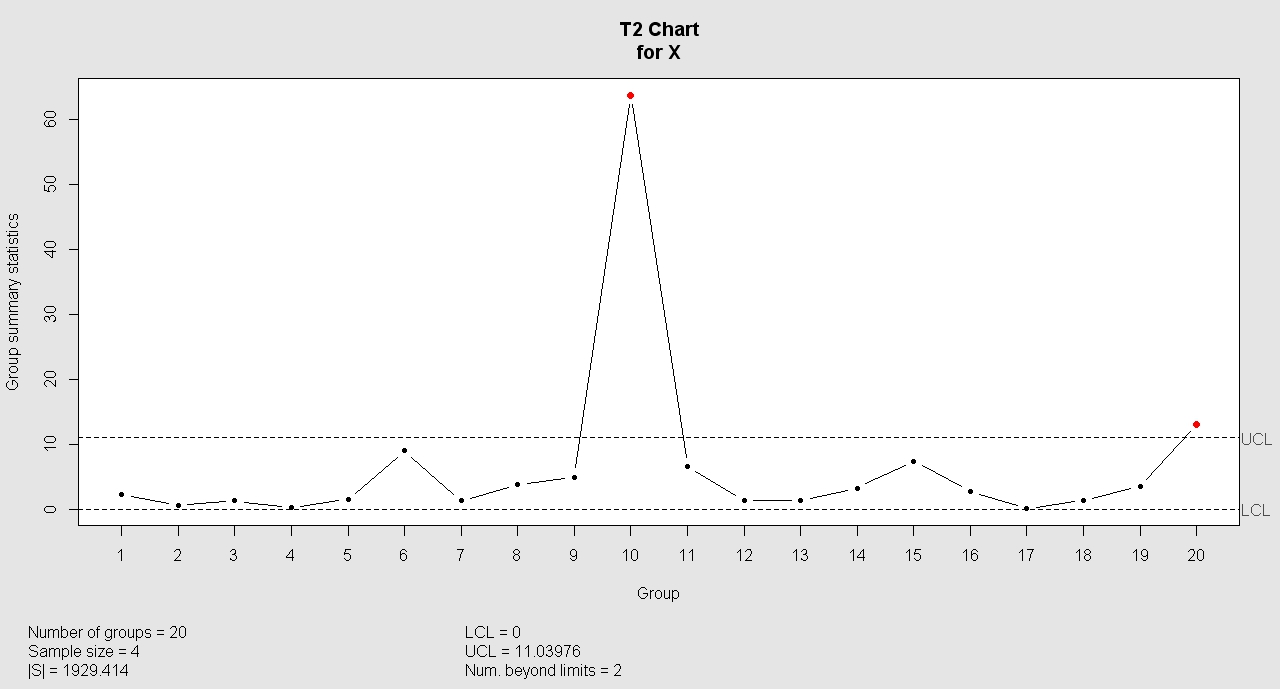
\includegraphics[width=0.9\linewidth]{./mqccplot1}
\caption{}
\label{fig:mqccplot1}
\end{figure}
\newpage
\begin{verbatim}
Call:
mqcc(data = X, type = "T2")

T2 chart for X 

Summary of group statistics:
   Min. 1st Qu.  Median    Mean 3rd Qu.    Max. 
 0.1243  1.3250  2.5030  6.4700  5.3490 63.7600 

Number of variables:  2
Number of groups:  20
Group sample size:  4

Center: 
     X1      X2 
60.3750 18.4875 

Covariance matrix:
         X1        X2
X1 222.0333 103.11667
X2 103.1167  56.57917
|S|:  1929.414 

Control limits:
 LCL      UCL
   0 11.03976

\end{verbatim}
\newpage
\section{Piston Rings (qcc package)}

\begin{figure}[h!]
\centering
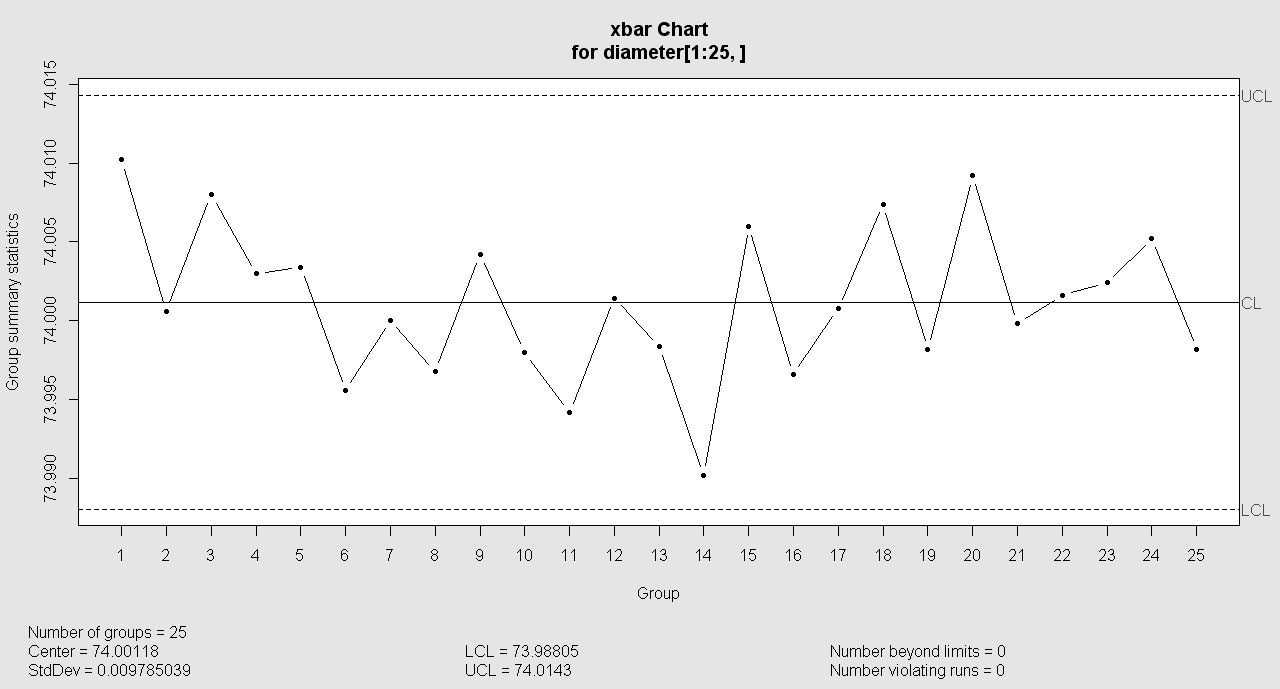
\includegraphics[width=0.7\linewidth]{./qccpistonrings-control}
\caption{}
\label{fig:qccpistonrings-control}
\end{figure}
\begin{figure}[h!]
\centering
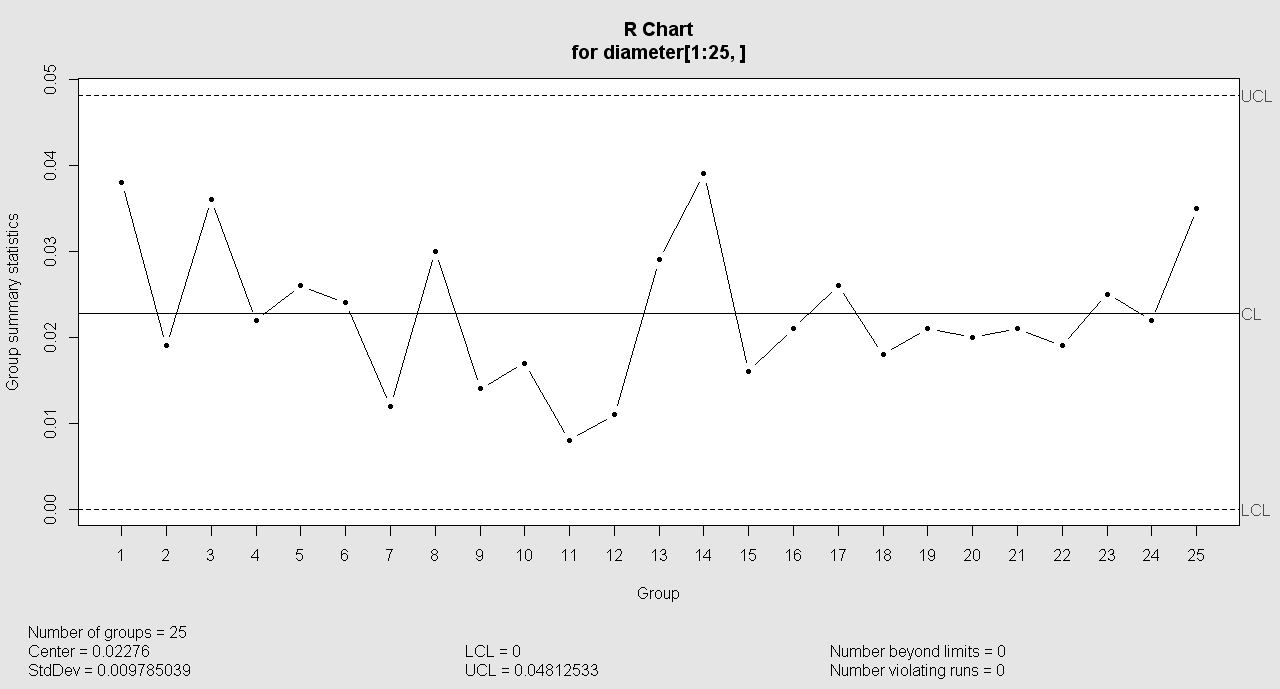
\includegraphics[width=0.7\linewidth]{./qccpistonrings-rchart}
\caption{}
\label{fig:qccpistonrings-rchart}
\end{figure}
\newpage
\begin{figure}[h!]
\centering
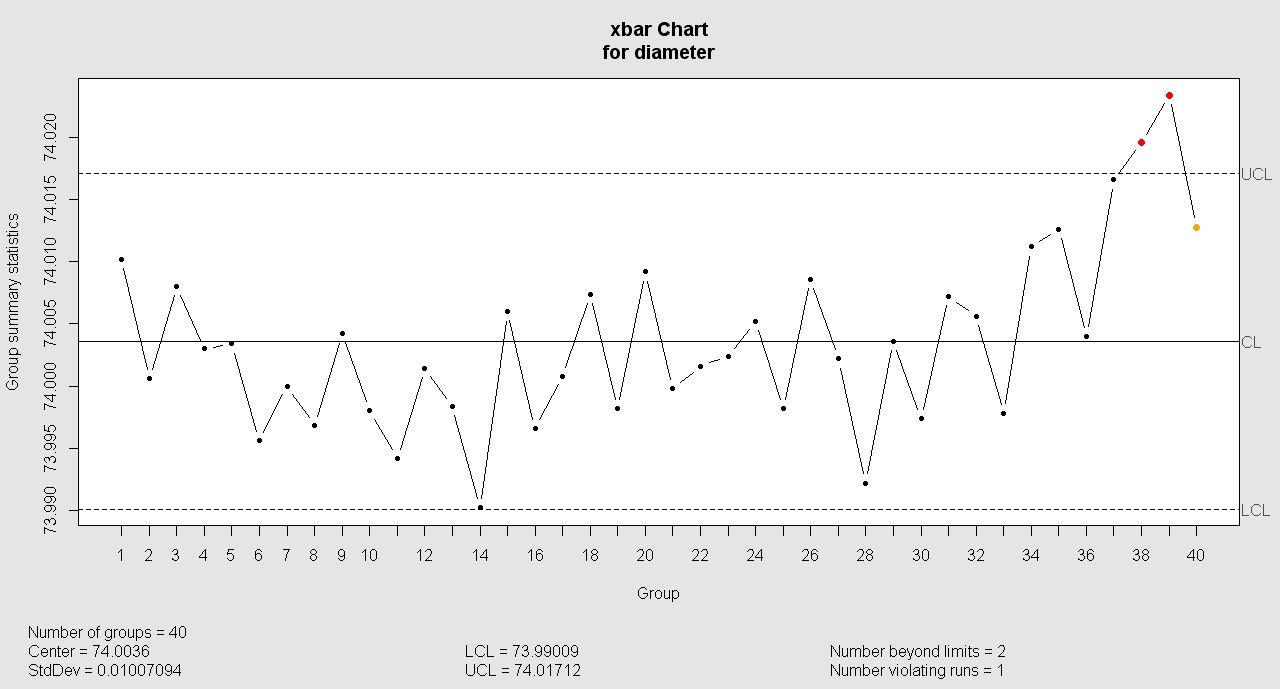
\includegraphics[width=0.7\linewidth]{./qccpistonrings-xbar2}
\caption{}
\label{fig:qccpistonrings-xbar2}
\end{figure}
\begin{figure}[h!]
\centering
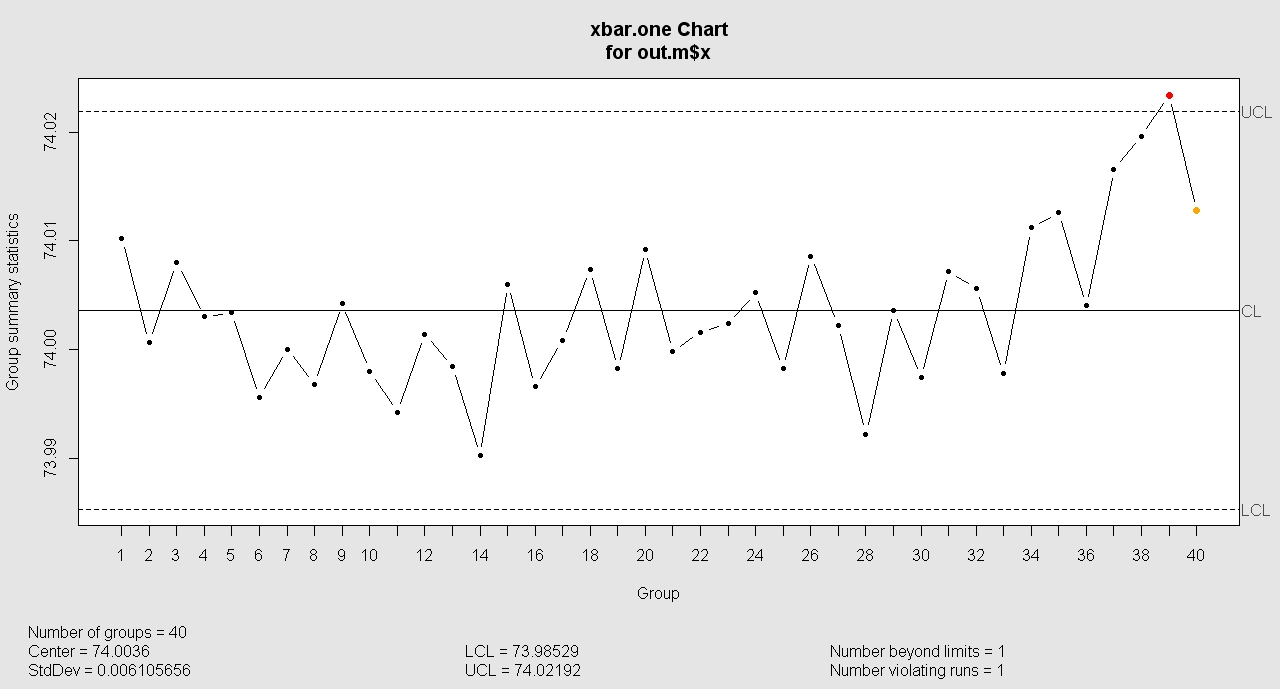
\includegraphics[width=0.7\linewidth]{./qccpistonrings-xbarone}
\caption{}
\label{fig:qccpistonrings-xbarone}
\end{figure}



\end{document}